

\chapter{Use Cases for Reactive Information Systems}
We have so far introduced a conceptual model for reactive information systems and their services.
Through our model we are able to react on events happening in \textrm{\glspl{infosystem}} and dispatch changes to it or any other accessible \textrm{\glspl{infosystem}}.
In this chapter we will give examples of what use cases can be realized through our model.

\section{Reacting on changes in the \gls{www}}
Many documents of the \textrm{\gls{www}} are dynamic in the way that they change over time.
Some might change in an interval of a few minutes (e.g. news), while others change much slower, such as knowledge sites.
To detect such changes an \textrm{\gls{infosystem}} in the \textrm{\gls{web}} needs to keep track of the document history and trigger events if there is a change.
In our model this would be realized by an \textrm{Event Trigger} which monitors a certain set of \textrm{\glspl{infospace}} and triggers events as soon as differences are detected.
A user will then set up a rule that checks if the changes are related to a certain category of interest, such as sports or a certain observed site, and how big those changes are.
If for example a Wikipedia article changed in more than 10\% of its content this will be a reason for a moderator to look at it and should be entered as a task in the next free slot of his calendar, as shown in Figure \ref{fig:DetectChangesInTheWeb}.
\begin{figure}[!ht]
  \centering
  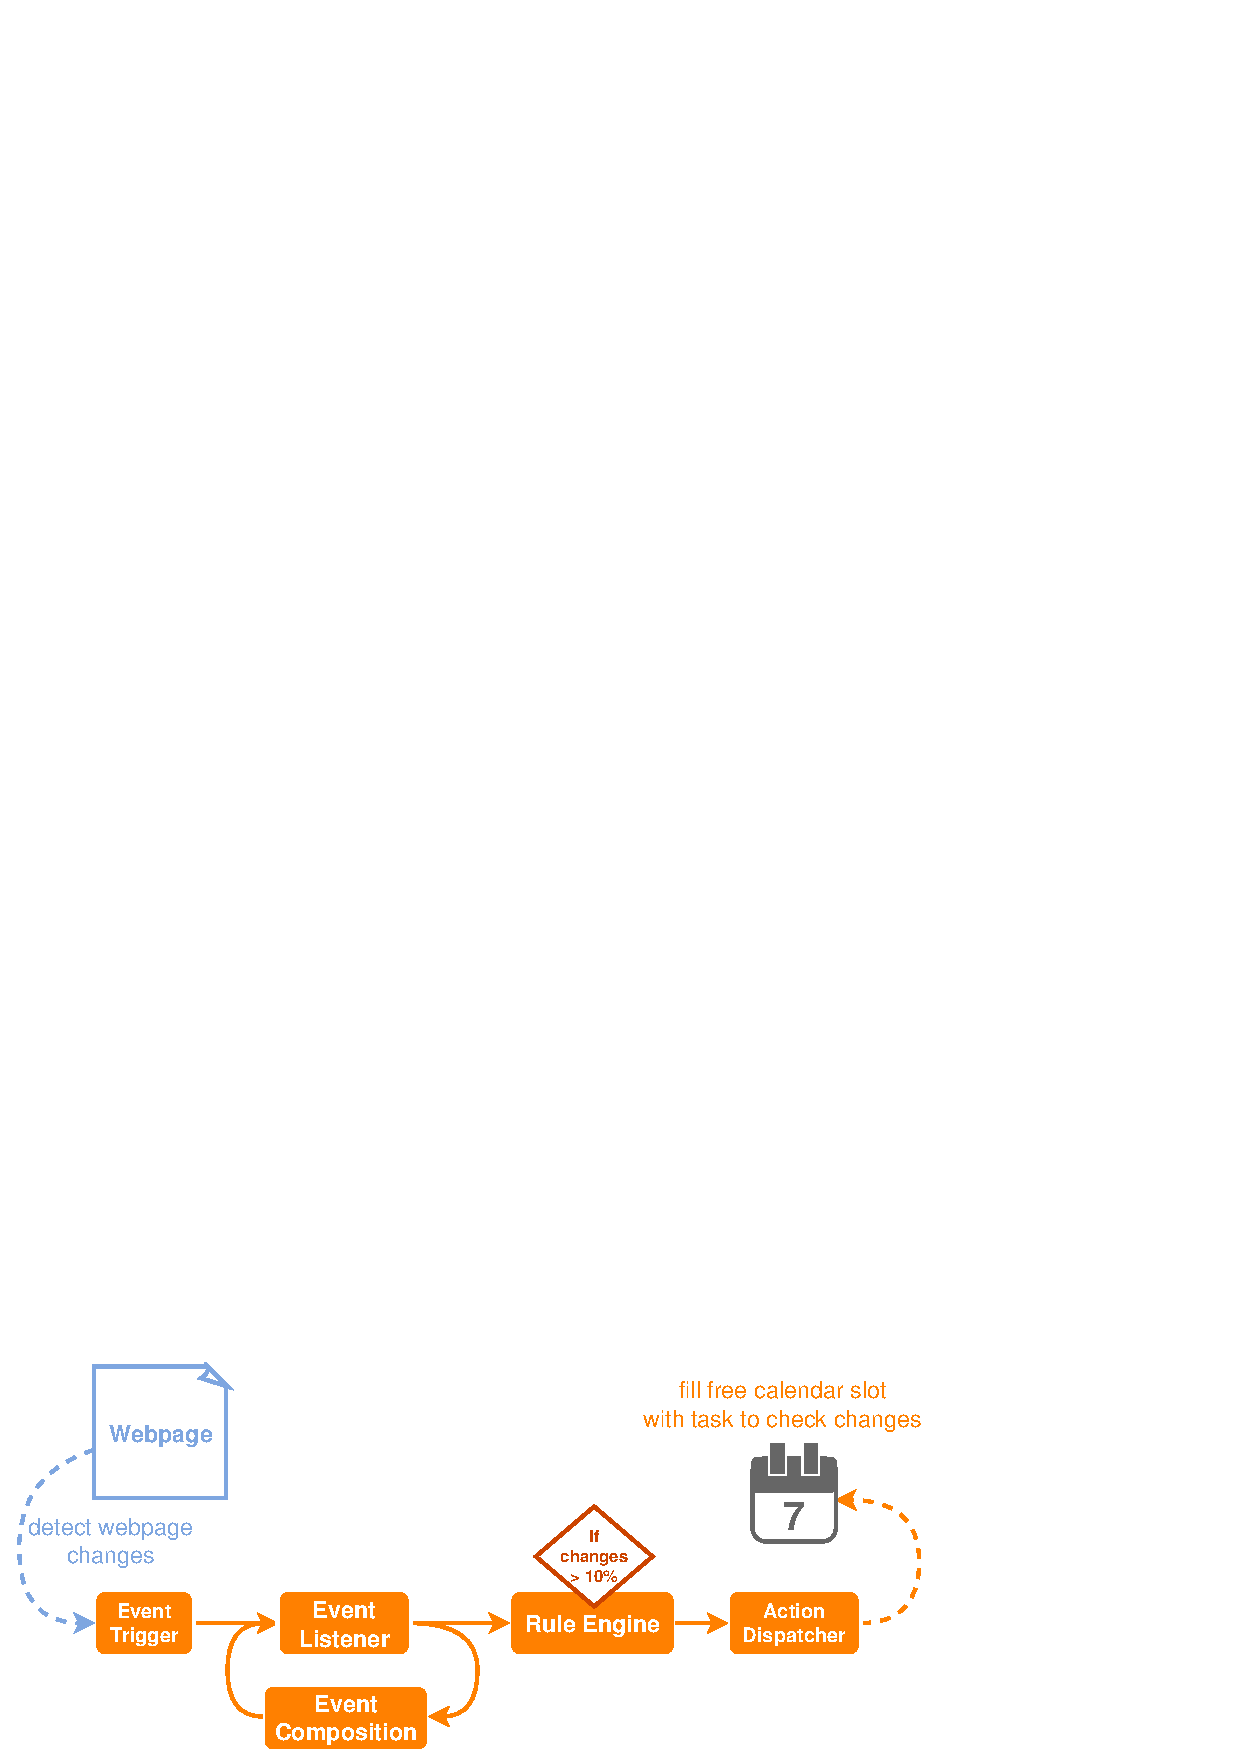
\includegraphics[width=0.8\textwidth]{figures/DetectChangesInTheWeb}
  \caption{Use Case; detect big changes in the \textrm{\gls{web}} and fill calendar slot of moderator with task}
  \label{fig:DetectChangesInTheWeb}
\end{figure}



\section{Enhance existing \glspl{webapplication}}
Web applications, such as webmails, social networks or \textrm{\acrlong{cms} (\acrshort{cms})} are widely spread and used by a large number of Internet users.
Users or developers often miss some features or interoperability with other web applications, which would result in enhanced functionality and also in less work.
Features of that kind could also include data and functionality from other \textrm{\gls{webresource}} on the web.
This would require \textrm{\glspl{webapplication}} to communicate together and to grab data or impose functionality upon each other.
A lot of enhancements will not be implemented by the \textrm{\glspl{webapplication}} themselves because they are very specific to a small number of their users.
With a reactive \textrm{\glspl{infosystem}}, users and developers could realize such features on their own.



\subsection{Enrich \acrlong{cms} Posts with Additional Information}
Every new post to a \textrm{\acrlong{cms}} can be modeled as an event.
In the case that a user would like to enrich such a \textrm{\acrshort{cms}} with knowledge from a remote resource, reactivity in the \textrm{\gls{web}} can be used to do it.
Enhancing an existing \textrm{\acrshort{cms}} can be realized by a rule that evaluates new posts and checks whether knowledge tags are included in the post, which is shown in Figure \ref{fig:ProBinderAnnotations}.
Whenever there are tags included within the post, the reactive entity will enrich the post with additional knowledge to these tags from a remote \textrm{\gls{webresource}} of the user's choice.
\begin{figure}[!ht]
  \centering
  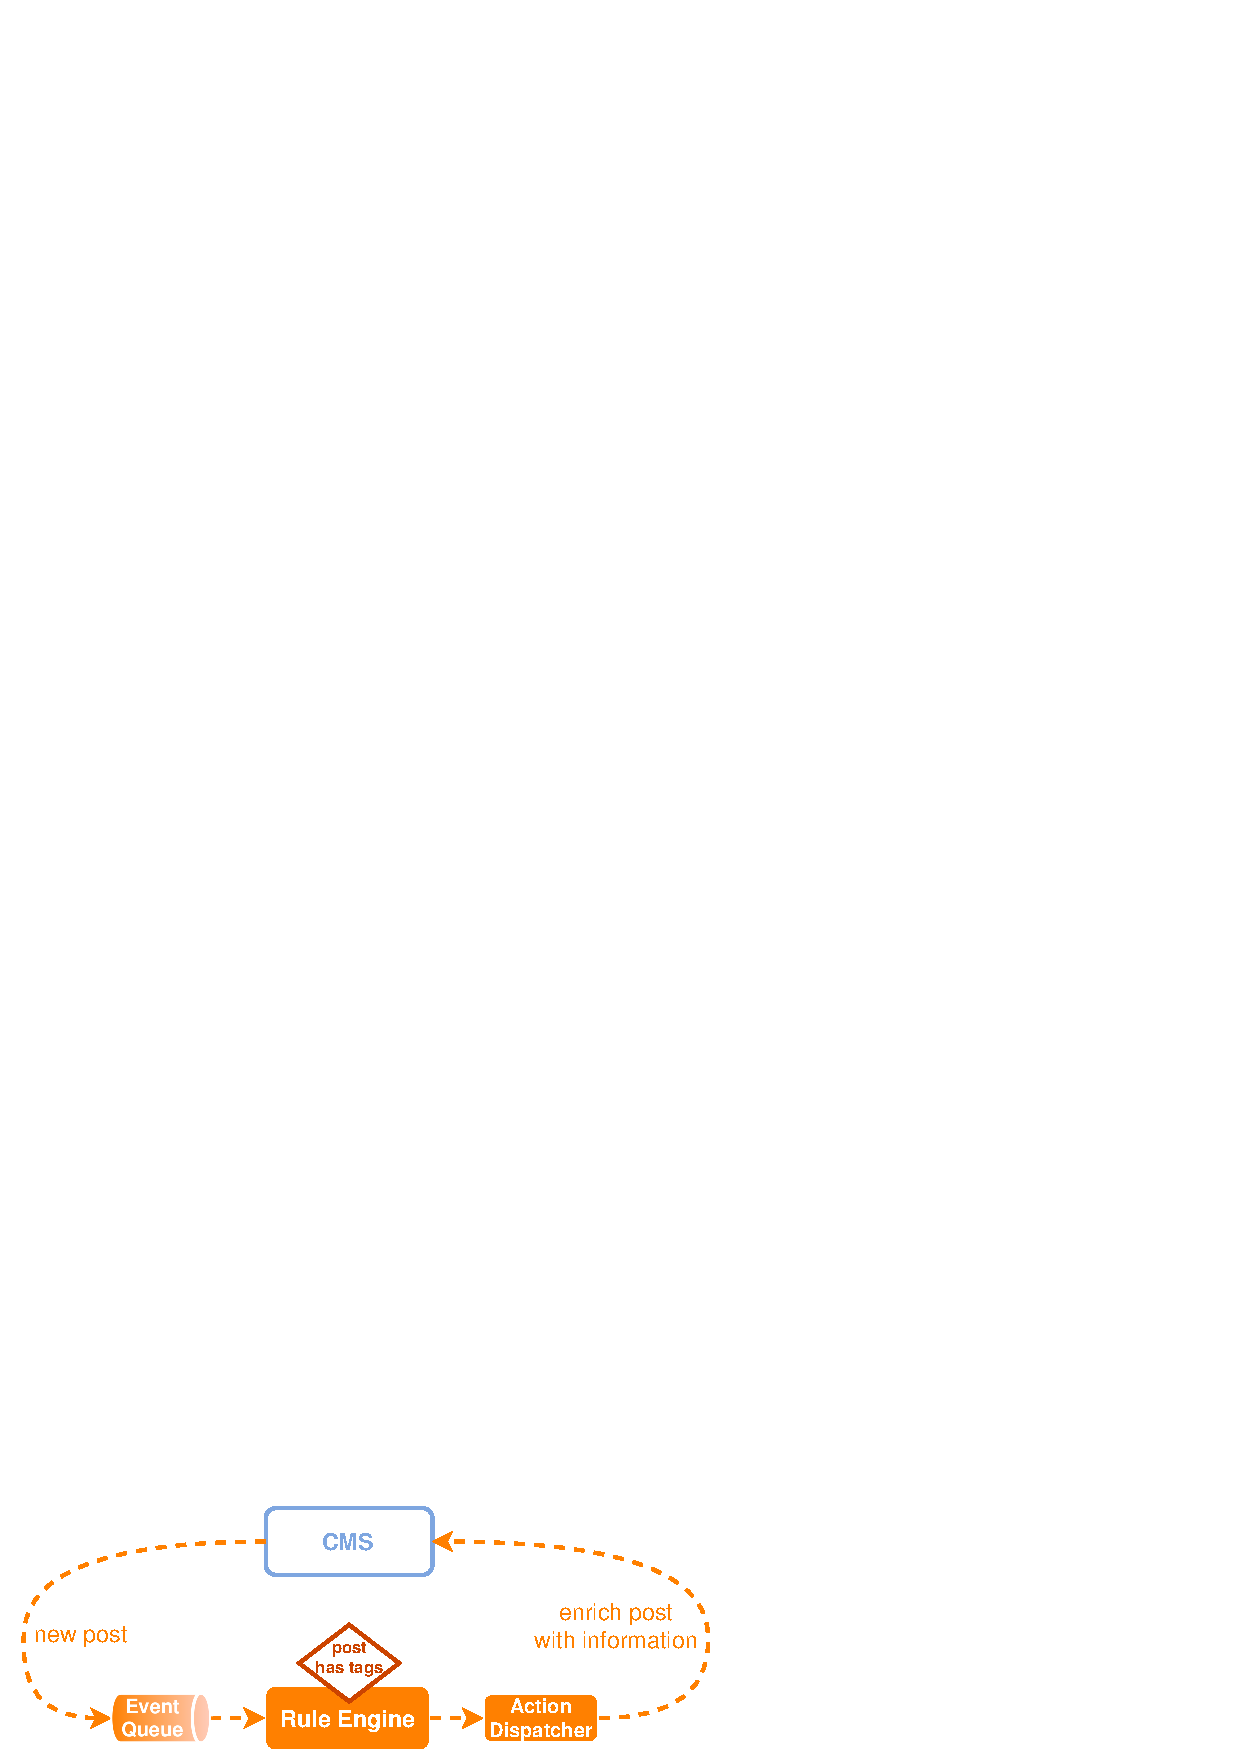
\includegraphics[width=0.8\textwidth]{figures/ProBinderAnnotations}
  \caption{Use Case; enrich \acrshort{cms} post with remote knowledge data}
  \label{fig:ProBinderAnnotations}
\end{figure}



\subsection{Workflow Automation}
Within such \textrm{\glspl{webapplication}}, users often have very specific workflows.
And because workflows always start with an event, they are predestined to be automated by a reactive entity.
As an example for workflow automation, course and student exercise submission administration can be taken care of by a reactive entity.
Figure \ref{fig:ProBinderCourseSetup} shows that whenever a new semester starts, the reactive entity will detect this through one of its rules and command an action dispatcher to set up infrastructures for courses.
This can also include grabbing course data from an official webpage and including it into the infrastructure, thus eliminating the need for manual data copy tasks.
\begin{figure}[!ht]
  \centering
  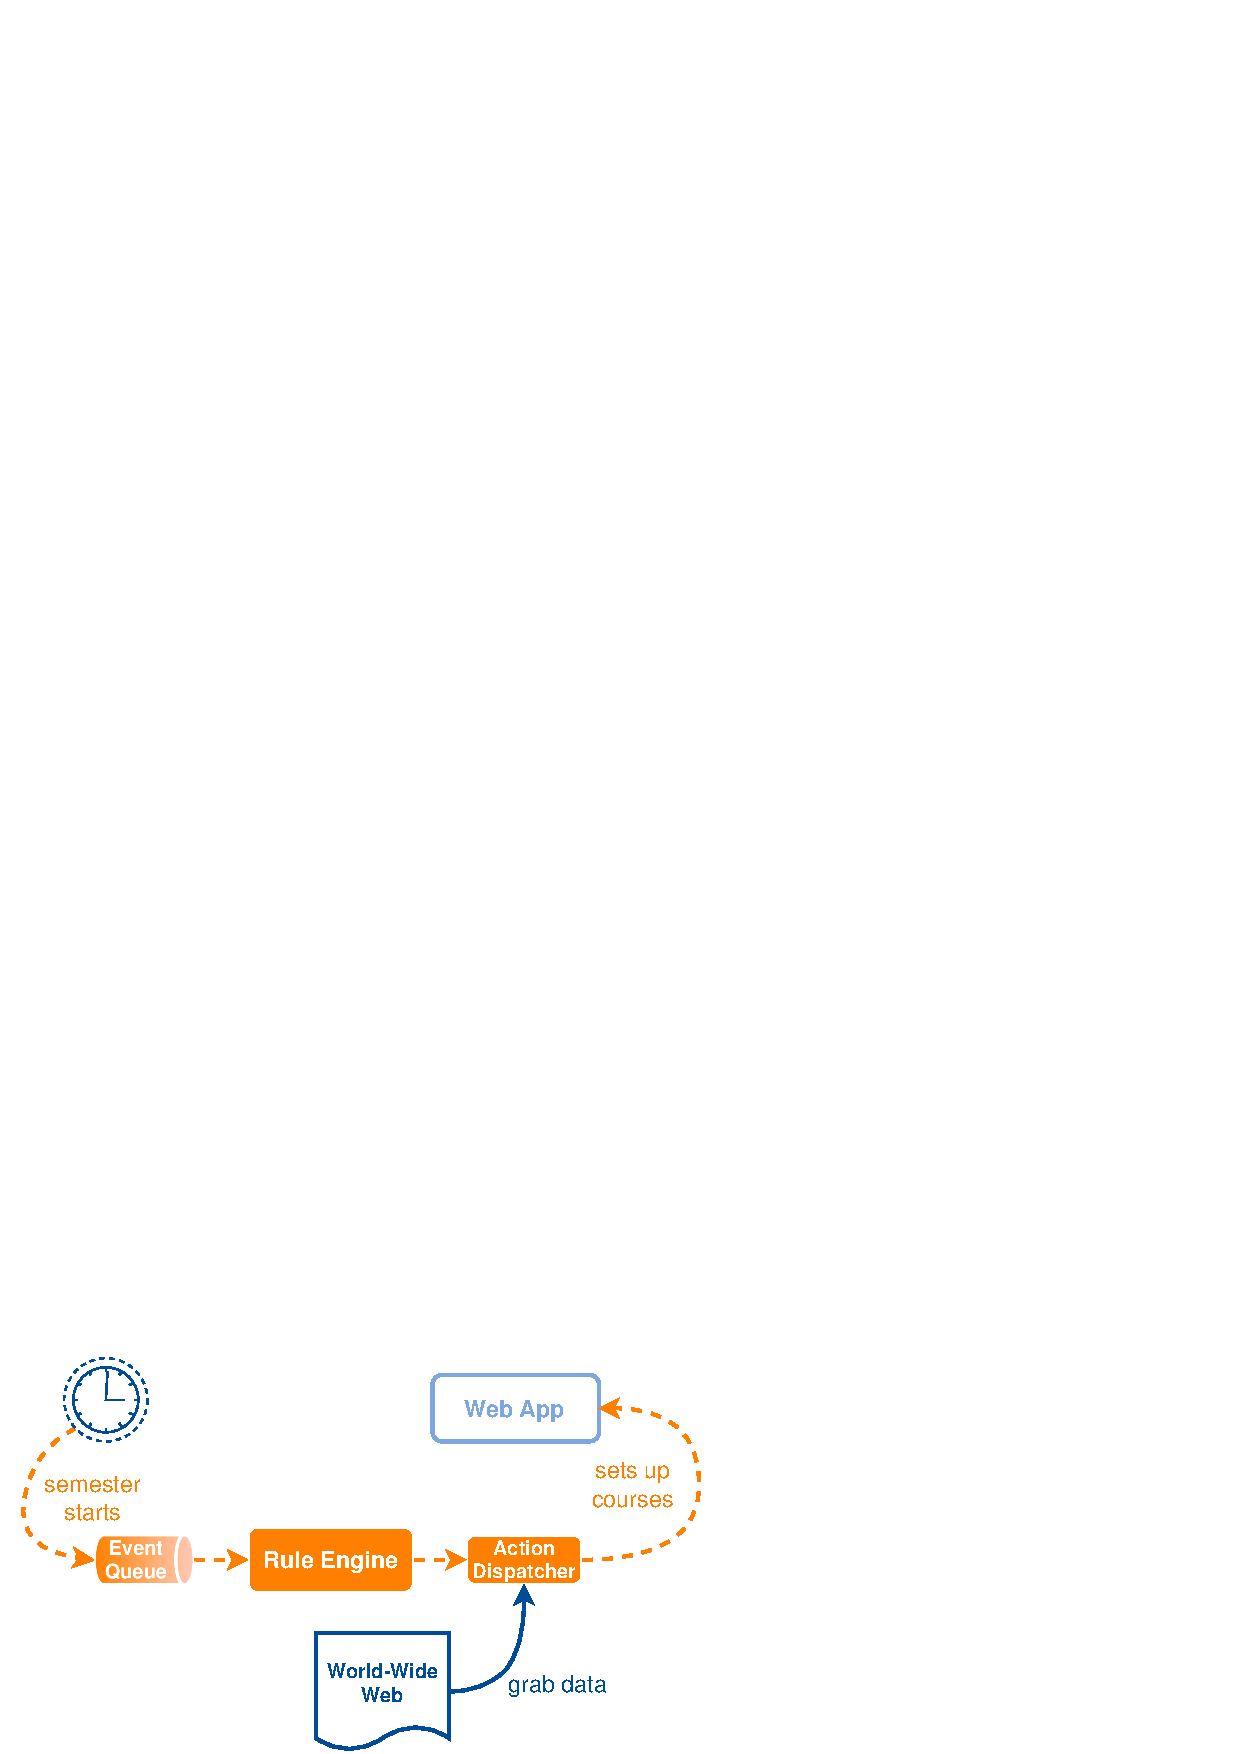
\includegraphics[width=0.8\textwidth]{figures/ProBinderCourseSetup}
  \caption{Use Case; create course resources at semester start}
  \label{fig:ProBinderCourseSetup}
\end{figure}

After setting up the semester courses, the reactive system is ready to process new student registrations for these courses.
It automatically associates students into the afore mentioned infrastructures and sets up additional infrastructure such as an exercise submission container.
Whenever a course tutor submits a new exercise to the course resource, the system will detect this and spread this information to the students, together with a deadline, as depicted in Figure \ref{fig:ProBinderStudentRegisters}.
The students are expected to submit their exercise solutions before the deadline, to the exercise submission container, which was created reactively for them.
\begin{figure}[!ht]
  \centering
  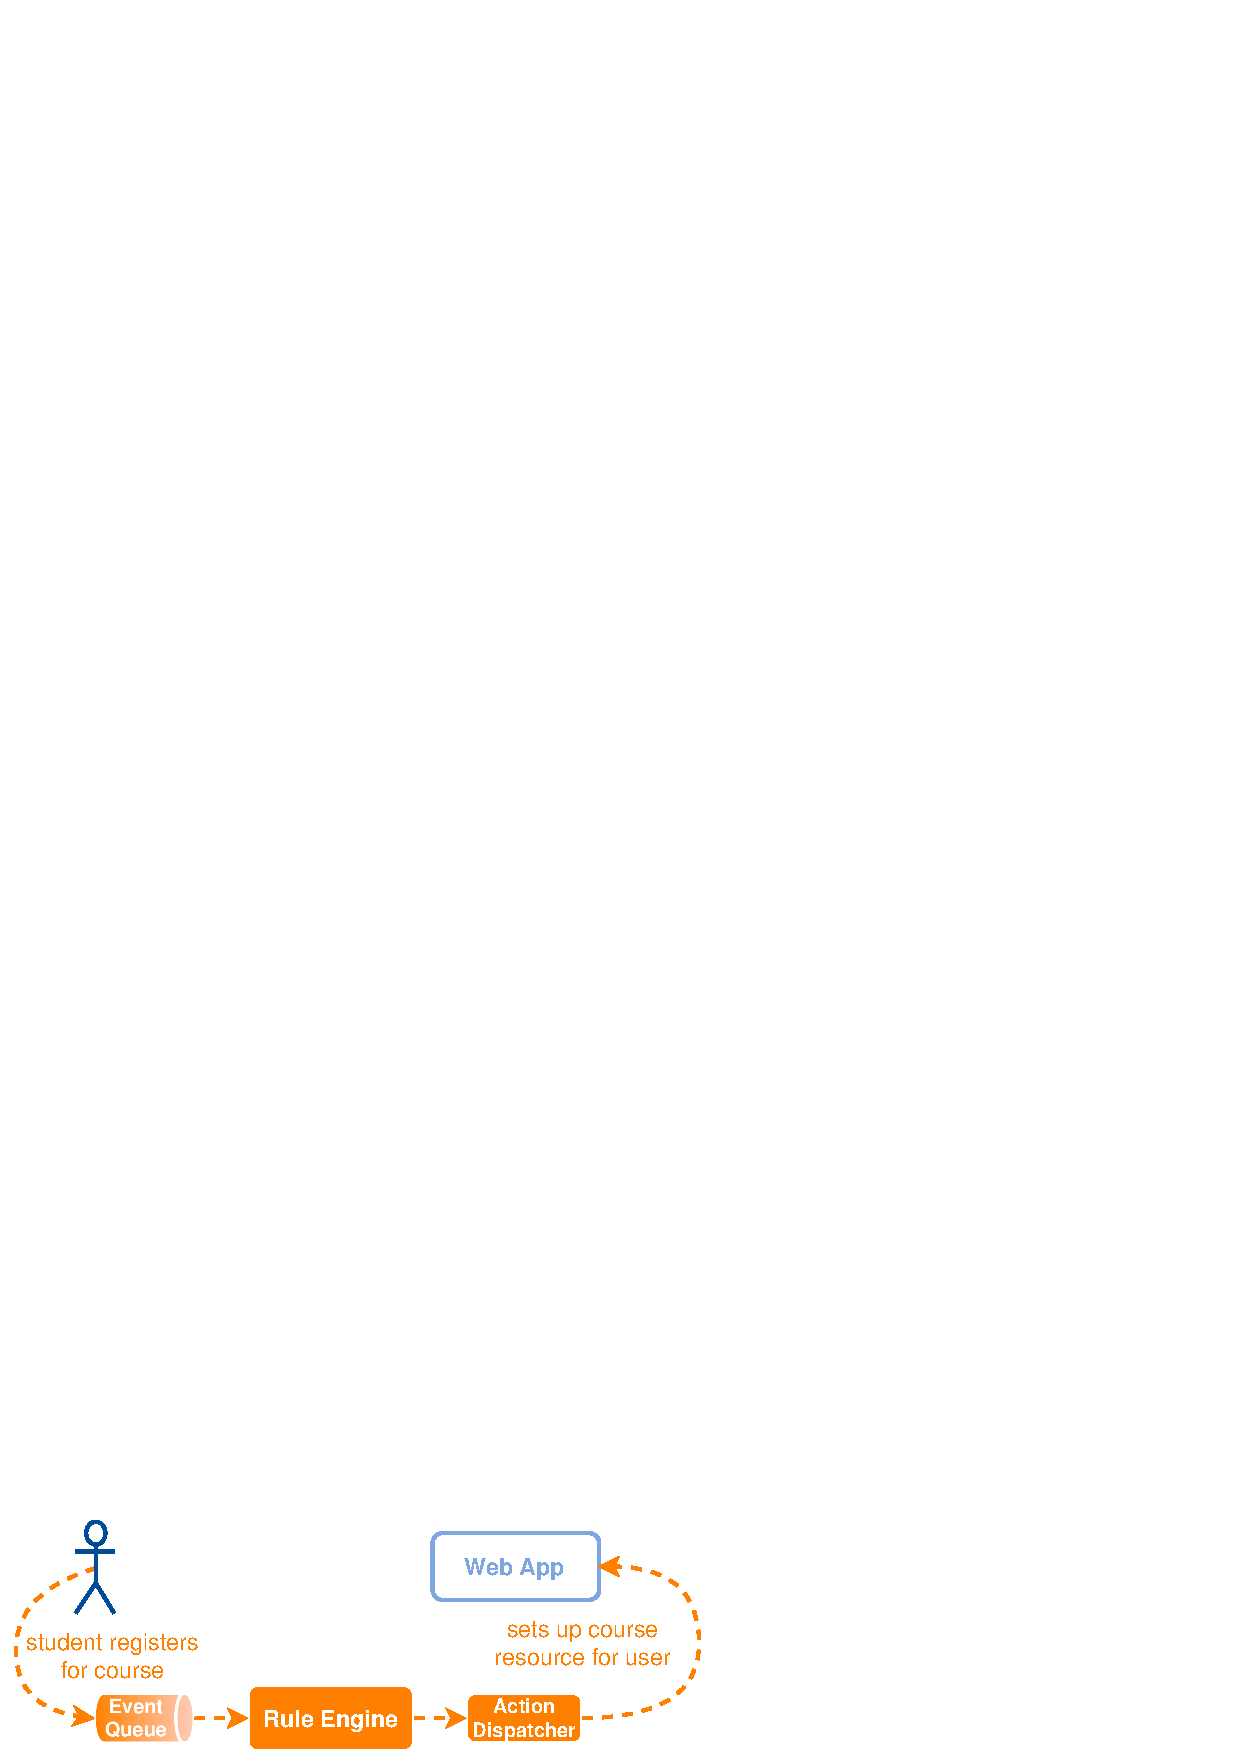
\includegraphics[width=0.8\textwidth]{figures/ProBinderStudentRegisters}
  \caption{Use Case; create course resource for registered student}
  \label{fig:ProBinderStudentRegisters}
\end{figure}

A certain amount of time before the deadline, e.g. one day, the reactive entity will detect the deadline and process events that depict the current exercise submission status per student.
If the system detects students who have not uploaded their exercises yet, it will notify them about the deadline, which is shown in Figure \ref{fig:ProBinderExerciseNotification}.
This is an additional service that gives students the chance to react on a missed exercise submission deadline.
As soon as the deadline passed, the system will revoke write-rights to the exercise submission container and therefore disallow submissions which are too late.
\begin{figure}[!ht]
  \centering
  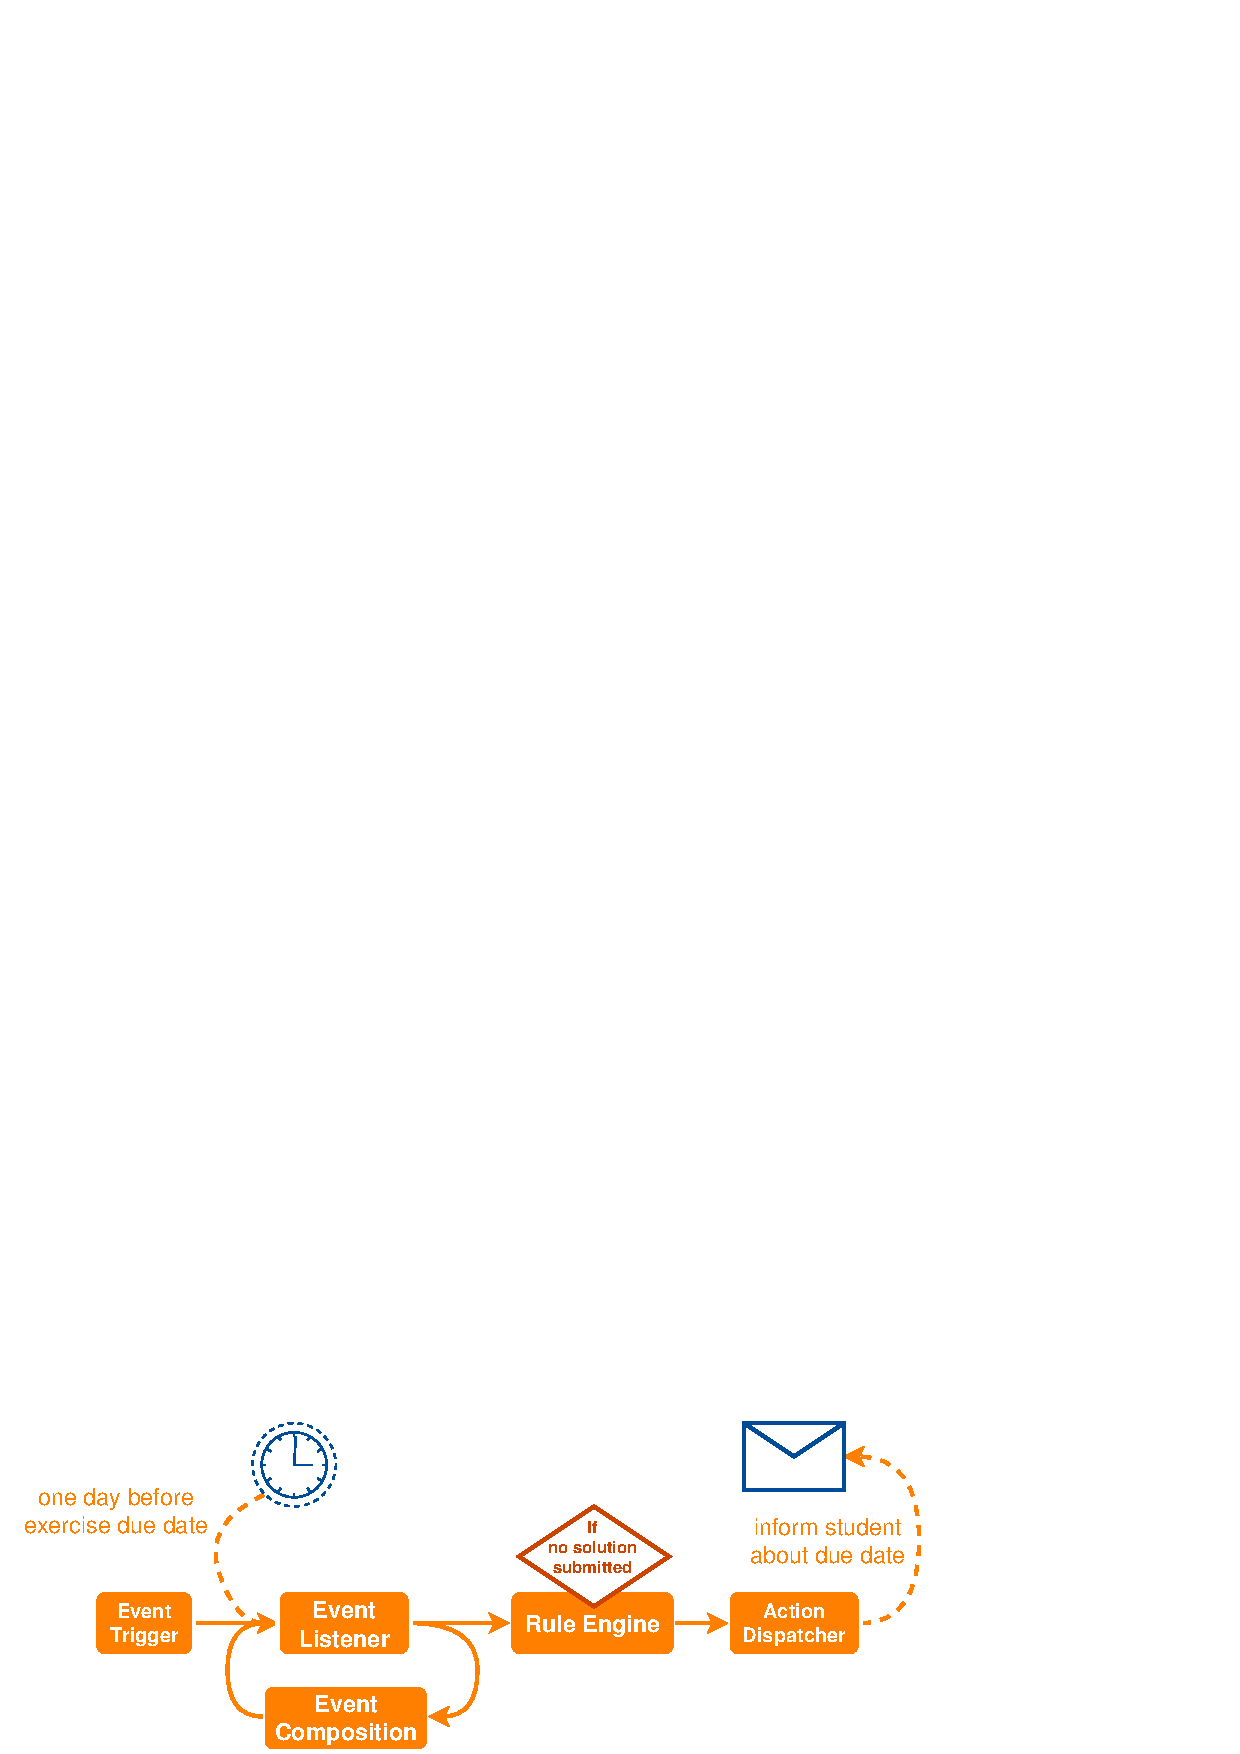
\includegraphics[width=0.8\textwidth]{figures/ProBinderExerciseNotification}
  \caption{Use Case; notify student before exercise due date}
  \label{fig:ProBinderExerciseNotification}
\end{figure}



\section{Service Functionality and Availability Checking}
Services offered through the \textrm{\gls{web}} are not monitored or tested by users or developers from other sites.
If they rely on correct functionality or availability they need a way to assert this.
It is also possible that an owner of such a service does not have the tools to monitor his own services.
Whenever such a service is not working correctly anymore or stops responding, these users or developers need to be able to react contemporary on this.
With a reactive rule in place that evaluates Service Testing results, countermeasurements can be taken early.
One action to such a failing service test could be an automatic switching of the utilized service within an action dispatcher, so that from then on it uses one which still works correctly, as shown in Figure \ref{fig:ProBinderServiceTesting}.
\begin{figure}[!ht]
  \centering
  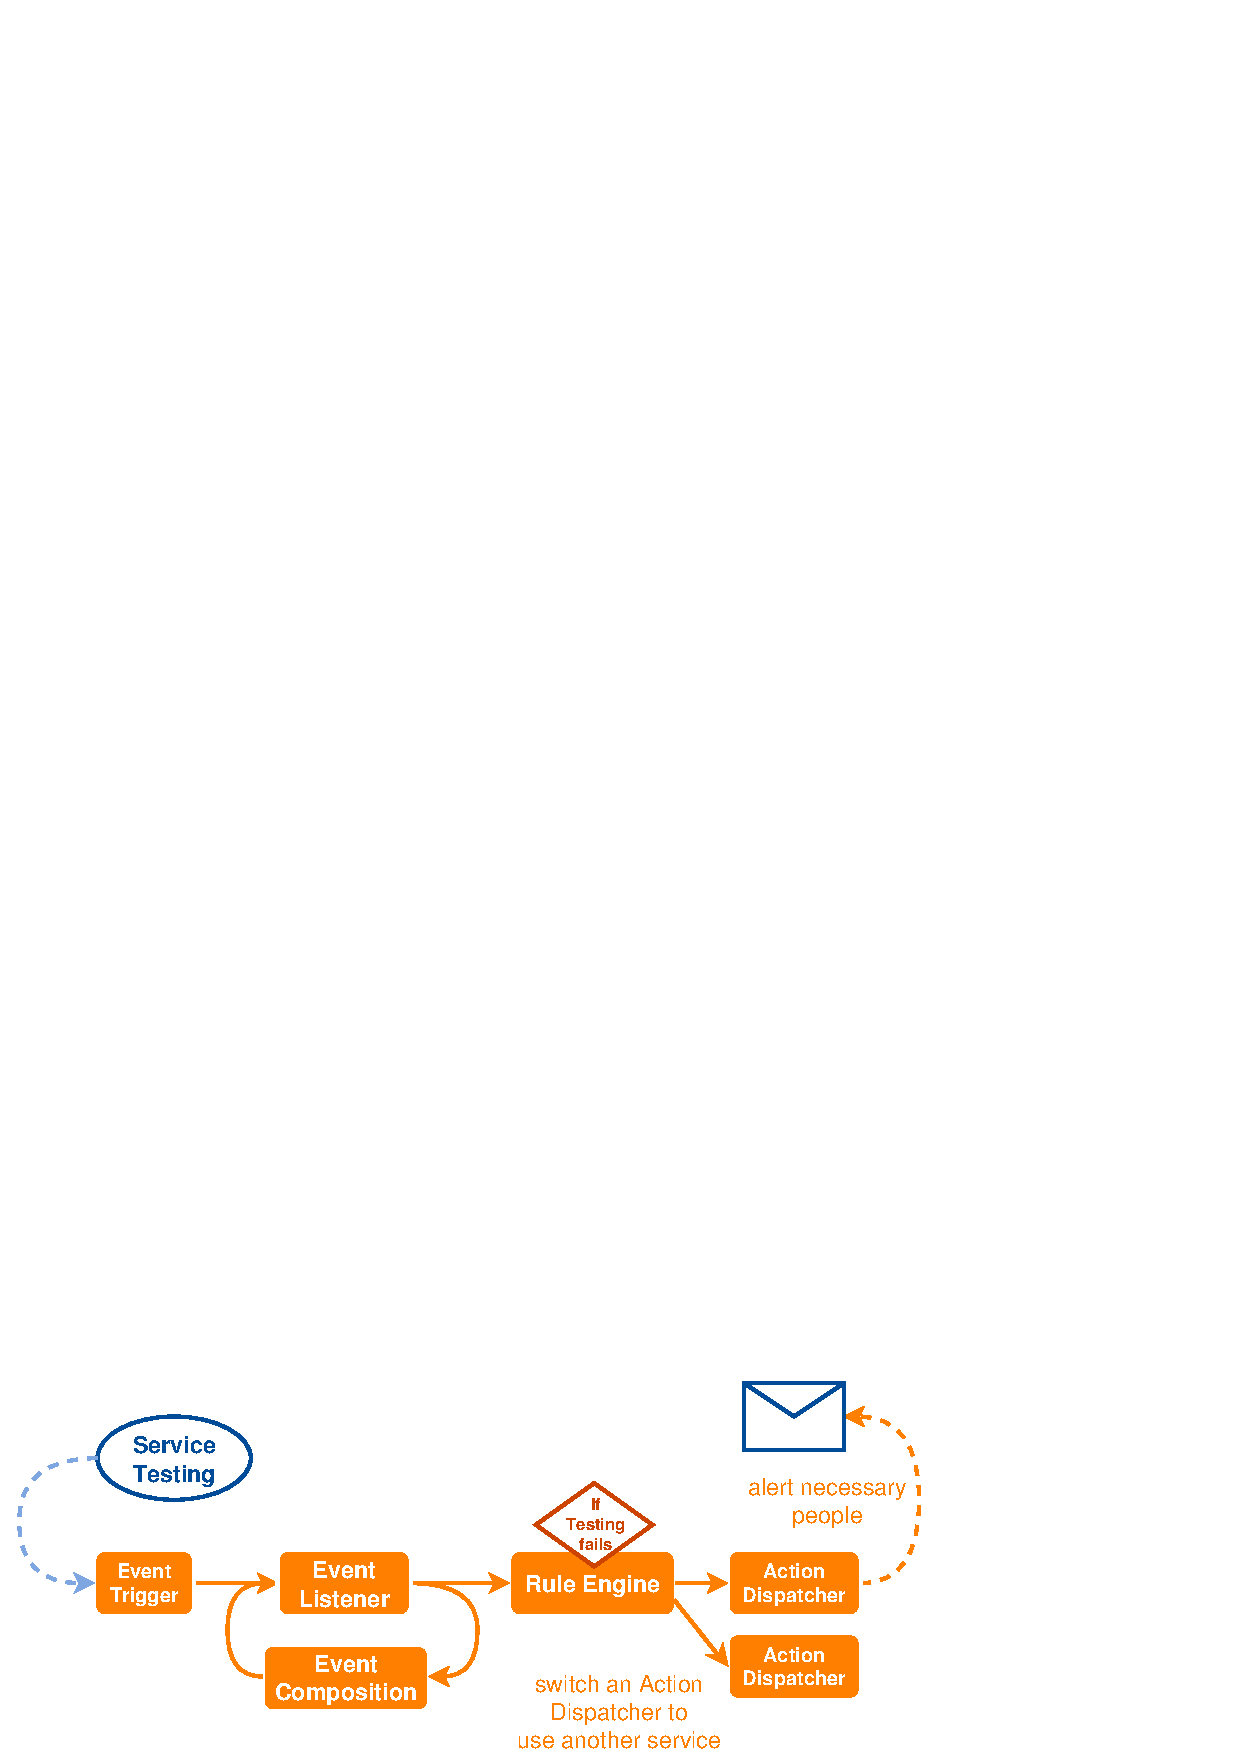
\includegraphics[width=0.8\textwidth]{figures/ProBinderServiceTesting}
  \caption{Use Case; test proper service functionality and availability}
  \label{fig:ProBinderServiceTesting}
\end{figure}



\section{Exploiting the \gls{webofthings}}
A model for reactive information systems becomes especially interesting in the context of the \textrm{\gls{webofthings}}. 
Through the small connected devices, a lot of sensor data become accessible via the \textrm{\gls{web}} and can be used as events to trigger actions.
These actions could also be part of the \textrm{\gls{webofthings}}, if there are such things, that offer services.
One example of a reactive rule, that has parts in the \textrm{\gls{webofthings}}, is that of a server room which has a defective cooling.
The increasing temperature eventually causes the servers to shutdown or even fail.
Servers in this room should push current state information into a reactive system.
The reactive system can then take countermeasures if it detects a certain pattern that will lead to an overheating of all systems.
It could inform certain (not so important) servers to gracefully shutdown and additionally inform administrators, who otherwise might miss the shutdown, as shown in Figure \ref{fig:WoT_Server}.
It would be even better, if such a system would have the power to enable an additional emergency cooling system to prevent the shutdown of any of the servers.
\begin{figure}[!ht]
  \centering
  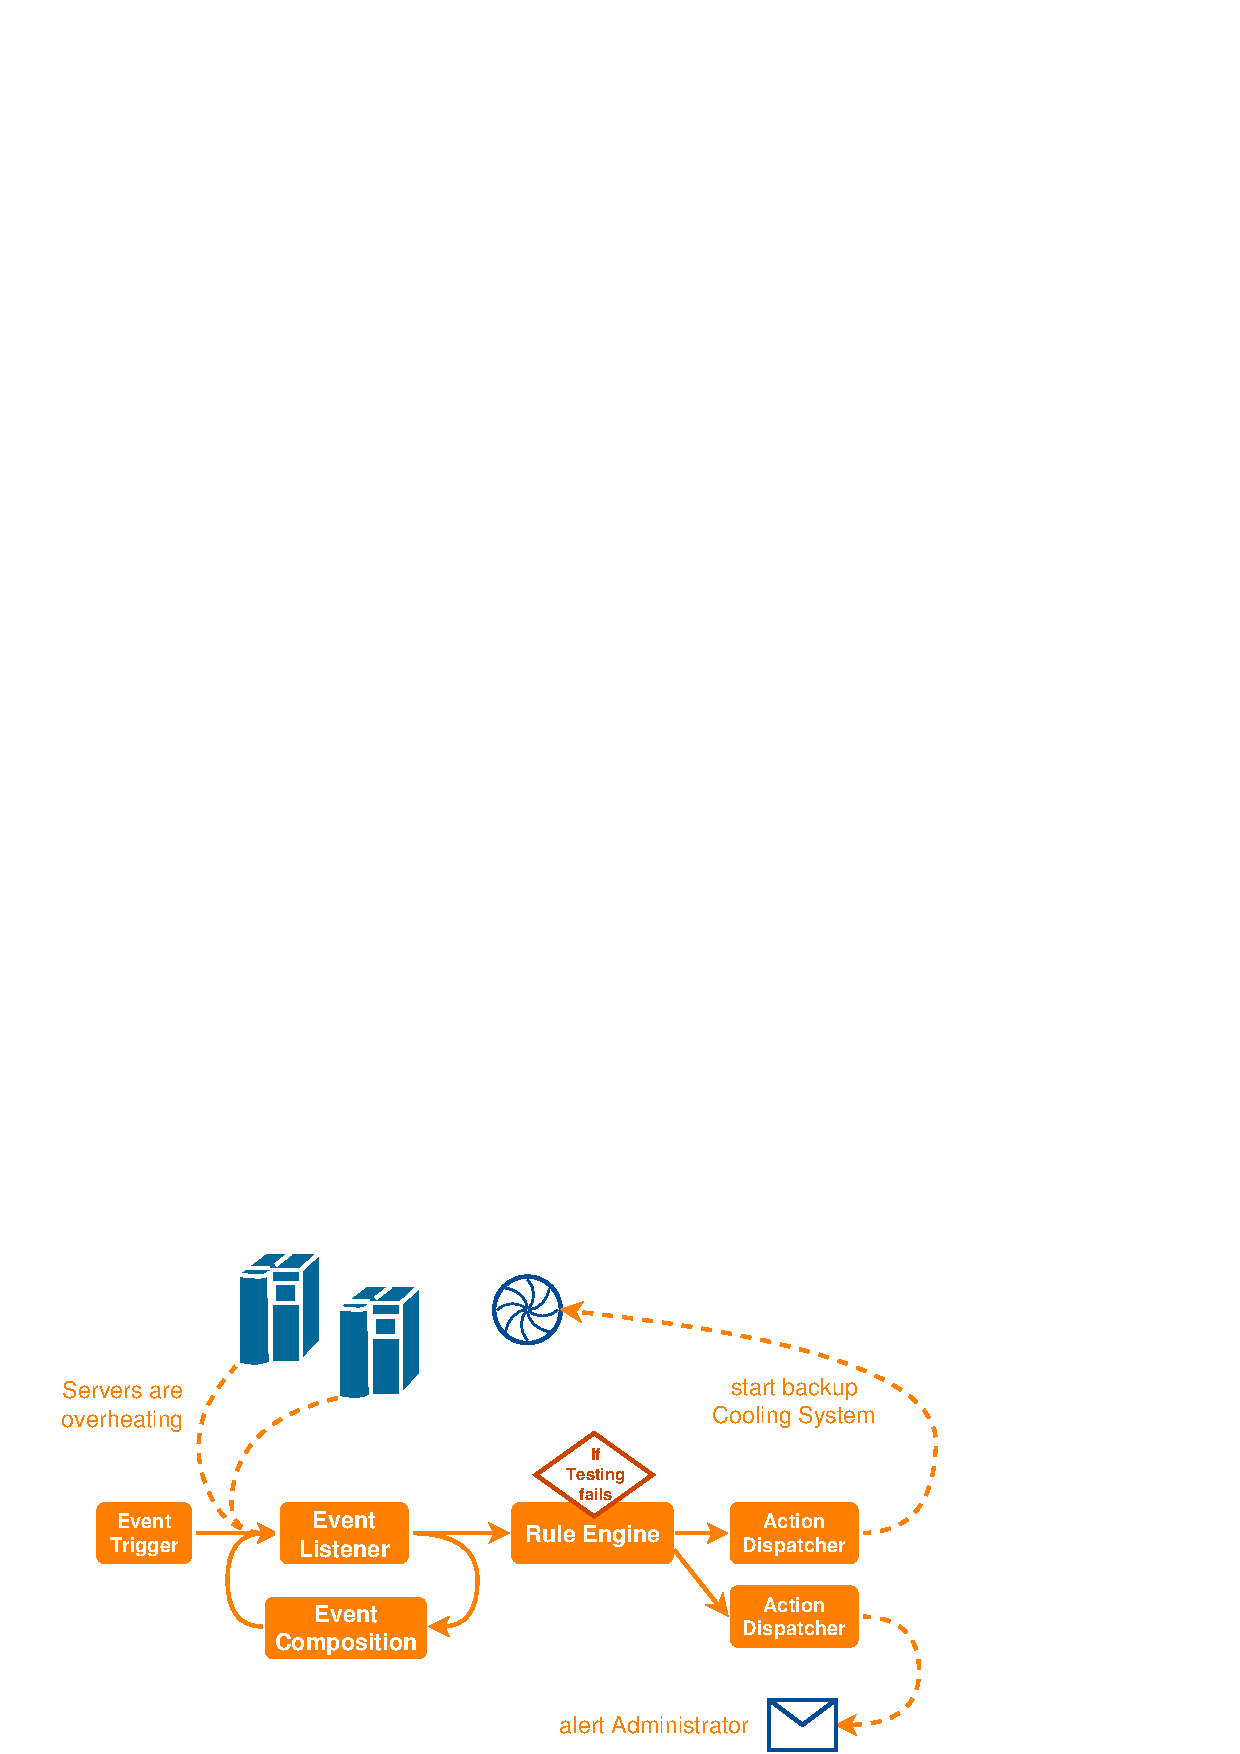
\includegraphics[width=0.8\textwidth]{figures/WoT_Server}
  \caption{Use Case; measurements on server failure}
  \label{fig:WoT_Server}
\end{figure}

Another scenario gets more realistic with the increasing number of homes that are connected to the Web.
A home or apartment owner has her light controls attached to the Web.
The first thing a reactive system could do, is that it detects holidays in the owner's agenda and automatically sets the light control to somewhat reasonable random during her absence.
This would make suspicious characters, which are eventually interested in her wealth, think that he's still at home.
In combination with another thing, that is connected to the \textrm{\gls{web}} and always accompanies people, the cell phone, an even more interesting application scenario can be thought of.
The phone would push location information about the owner into the system.
Whenever the owner gets close to her house, the reactive system could turn on the light in the entry area and play some music.
On a Wednesday evening it could also inform the delivery service that they can deliver the owner's preferred menu when she is home, because the owner is doing this always on a Wednesday evening.



\section{Averaged Bad Weather Prediction}
There are a lot of different weather services existing in the Web.
One has to check several of them in order to get an idea on how likely it is that it will be raining on the journey to work and back.
By composing a higher-order event from several weather update events, a user could store a rule which alarms him early in the morning if more than 50\% of the weather forecasts expect rain on the way to or back from work.
% TODO refer to figure
